% Drawing 148/04-4 -- folder 148, batch 04, archive page 67 (PDF page 68).
% Transcription: esquisses au crayon, en haut à droite de la feuille : une boucle attachée à un sommet ; deux arêtes à deux sommets, chaque sommet entouré de petits cercles et l'arête entourée de courbes ovales ; un cercle portant six sommets ; un disque à deux trous reliés par une bande, avec des segments radiaux.
% Kind: pencil sketches: loop, edges with ringed vertices, circle with six vertices, disk with two holes. Method 2 (schematic redraw from the facsimile). Status: partial.
% Notes: Faint pencil on the back of a listing (seen with the contrast raised). Loop: one vertex with a closed curve leaving and returning, and a curved stroke inside it from the vertex. First edge: a heavy stroke between two points, its line drawn on thinly beyond both ends, a ring round each point, a long closed contour round the whole, and a stroke crossing the right ring. Second edge: a heavy stroke between two points, a ring round each, an oval contour round the whole. Circle with six vertices: an oval outline (doubled on the page, drawn once) with six points on it, three chords inside (from the upper left point to the right point, from the top point down to the bottom, and from the lower left point to the right point), and a faint outer loop at its upper left. Disk with two holes: an egg-shaped outline, two holes joined by a band of two strokes, and nine radial segments from the holes to the outline. The row of four small ink marks above the figures is left out (not read as a drawing), as are the typed lines of the listing. Redrawn 2026-11-12 (issue 128). 2026-11-13, Claude Opus 5.5, issue 147, overlay check: not compiled (no TeX in the session); the TikZ was rasterised by a local interpreter and laid over the 403 ppi scan rendered at 400 dpi, contrast raised. Redrawn on the ink: points on their blots, rings and the six-vertex oval fitted as ellipses, contours and outlines through points read on gridded crops or moved onto their ink. Changed: every figure moved onto the page (the earlier redraw was up to four units off); the line of the first edge drawn beyond its ends, the crossing stroke, the inner stroke of the loop, the three chords and the outer loop of the six-vertex circle added; the band and the radial segments drawn where they are. Still differs: the pencil is so faint that the loop's right side and the disk's outline could only be followed to within about two units (the other figures lie on their ink to within about one unit); the radial segments of the disk are read from a 20 px per unit crop and may be a stroke or so short of the page's count.
% Coordinates: 1 unit = 1 mm = 1/100 of the crop width, y downwards as on the crop (bbox in page fractions: [0.55, 0.07, 0.95, 0.275]).
% Redrawn by Claude (claude-fable-5-2), issue #128, 2026-11-12; not checked by a human; not compiled (no TeX in the session); overlay-checked on the scan by Claude Opus 5.5, issue #147, 2026-11-13, not compiled (no TeX in the session).
% Rights: reproduces part of the work -- behind RENDER_TRANSCRIPTS, never published by itself.
\documentclass[tikz,border=3pt]{standalone}
\usepackage{amsmath,amssymb}
\usetikzlibrary{patterns,arrows.meta}
\tikzset{pencil/.style={black!45}, struck/.style={black!35}, mpt/.style={circle,draw,inner sep=1.3pt}, pt/.style={circle,fill,inner sep=0.9pt}, opt/.style={circle,draw,fill=white,inner sep=1.1pt}, Rd/.style={red!75!black}, Gn/.style={green!45!black}, Br/.style={brown!70!black}}
\begin{document}
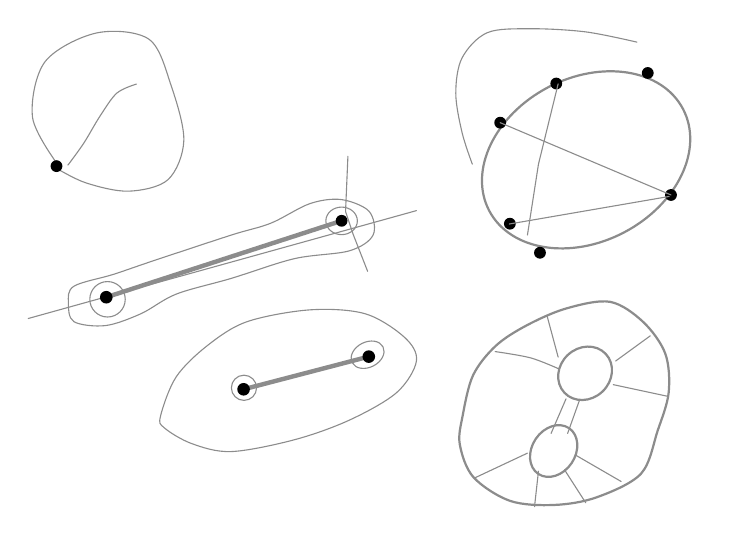
\begin{tikzpicture}[x=1mm,y=-1mm,line cap=round,line join=round,font=\small]
% loop: one vertex with a closed curve leaving and returning
\draw[pencil] plot[smooth, tension=0.55] coordinates {(17.82,25.87) (14.74,20.01) (16.34,12.98) (22.86,9.34) (29.54,10.14) (32.36,16.06) (33.96,23) (31.96,27.96) (26.98,29.43) (21.54,28.38) (17.55,26.39)};
\draw[pencil] plot[smooth, tension=0.55] coordinates {(19.24,26.12) (21.25,23.34) (23.32,19.89) (25.46,16.97) (27.95,15.83)};
\fill (17.79,26.25) circle [radius=0.75];
% first edge: a heavy stroke between two points, its line drawn on beyond both, a ring round each point, a long closed contour round it, and a stroke crossing the right ring
\draw[pencil] (14.2,45.6) -- (63.5,31.9);
\draw[pencil,line width=1.6pt] (24.11,42.9) -- (54,33.19);
\fill (24.11,42.9) circle [radius=0.8];
\fill (54,33.19) circle [radius=0.75];
\draw[pencil] (24.27,43.16) circle [radius=2.25];
\draw[pencil] (54,33.2) ellipse [x radius=2, y radius=1.75];
\draw[pencil] plot[smooth cycle, tension=0.55] coordinates {(20,41.5) (25,40) (30,38.3) (40,35) (45,33.5) (50,31) (54,30.5) (57.5,32) (58,35) (55,37) (48,38) (40,40.5) (33,42.5) (28.5,45) (24,46.5) (20,46) (19.3,43.6)};
\draw[pencil] (54.8,25) -- (54.5,32) -- (55.5,35) -- (57.3,39.6);
% second edge: a heavy stroke between two points, a ring round each, an oval contour round it
\draw[pencil,line width=1.6pt] (41.55,54.59) -- (57.45,50.44);
\fill (41.55,54.59) circle [radius=0.8];
\fill (57.45,50.44) circle [radius=0.8];
\draw[pencil] (41.6,54.4) circle [radius=1.6];
\draw[pencil,rotate around={26.9:(57.3,50.2)}] (57.3,50.2) ellipse [x radius=2.2, y radius=1.6];
\draw[pencil] plot[smooth cycle, tension=0.55] coordinates {(31,58) (33,53) (37,49) (42,46) (50,44.5) (57,45) (62,48) (63.5,51) (61,55) (55,58.5) (48,61) (40,62.5) (35,61.5) (31.5,59.5)};
% circle with six vertices (doubled on the page, drawn once), three chords, a faint outer loop at its upper left
\draw[pencil,thick,rotate around={27.7:(85.05,25.45)}] (85.05,25.45) ellipse [x radius=13.9, y radius=10.4];
\foreach \p in {(74.14,20.73),(81.26,15.76),(92.88,14.42),(95.83,29.91),(75.37,33.56),(79.19,37.25)} {\fill \p circle [radius=0.75];}
\draw[pencil] (74.14,20.73) -- (95.83,29.91);
\draw[pencil] (81.5,15.8) -- (79,26) -- (77.6,35);
\draw[pencil] (75.3,33.6) -- (95.6,30.1);
\draw[pencil] plot[smooth, tension=0.55] coordinates {(91.5,10.5) (85,9.2) (78,8.8) (72.5,9.3) (69.3,12.5) (68.5,17) (69.3,22) (70.6,26)};
% disk with two holes joined by a band of two strokes, and radial segments from the holes to the outer circle
\draw[pencil,thick] plot[smooth cycle, tension=0.55] coordinates {(69.36,58.01) (70.69,52.82) (73.57,49.08) (77.49,46.48) (82.51,44.33) (88.08,43.48) (92.3,46.04) (95.11,50.07) (95.54,54.98) (94.14,59.84) (92.03,65.3) (86.41,68.3) (81,69.28) (75.39,68.76) (70.73,65.74) (69.01,61.59)};
\draw[pencil,thick,rotate around={43.2:(84.92,52.56)}] (84.92,52.56) ellipse [x radius=3.6, y radius=3.2];
\draw[pencil,thick,rotate around={56.1:(80.93,62.43)}] (80.93,62.43) ellipse [x radius=3.5, y radius=2.75];
\draw[pencil] (82.5,55.8) -- (80.6,60.2);
\draw[pencil] (84.2,56) -- (82.7,60.2);
\draw[pencil] (81.5,50.5) -- (80.1,45.3);
\draw[pencil] (88.8,51) -- (93.2,47.8);
\draw[pencil] (88.5,54) -- (95.5,55.5);
\draw[pencil] plot[smooth, tension=0.55] coordinates {(81.6,52) (78,50.6) (73.5,49.8)};
\draw[pencil] (77.6,62.7) -- (71,65.8);
\draw[pencil] (79,65) -- (78.5,69.5);
\draw[pencil] (82.3,64.8) -- (85,69);
\draw[pencil] (83.8,63) -- (89.5,66.3);
\end{tikzpicture}
\end{document}
